\authoredSection{corny}{Toolchain}
Im Rahmen unseres Projekts wurde uns schnell klar, dass wir auf viele Tools angewiesen sein würden. So musste unser Quelltext versioniert, die grobe Struktur und Views festgehalten und Aufgabenpakete erstellt und koordiniert werden. Darüber hinaus war uns auch Design und Qualität wichtig. Auf unsere Erfahrungen in diesem Zusammenhang gehen wir im folgenden Abschnitt ein.

\subsection{Agiles Vorgehen im Projekt}
	Da uns freundlicherweise von C1 WPS die Möglichkeit gegeben wurde, eine Scrum-Zertifizierung zu erhalten, lag uns viel daran, den Scrum-Ansatz so gut es ging in unseren Projekt-Ablauf zu integrieren. Dazu verwenden wir die Software PivotalTracker, in der wir zum einen, wie in Abbildung \ref{fig:TrackerStories} dargestellt, einzelne Stories administrieren können,
\begin{figure}[h!]
	\centering
	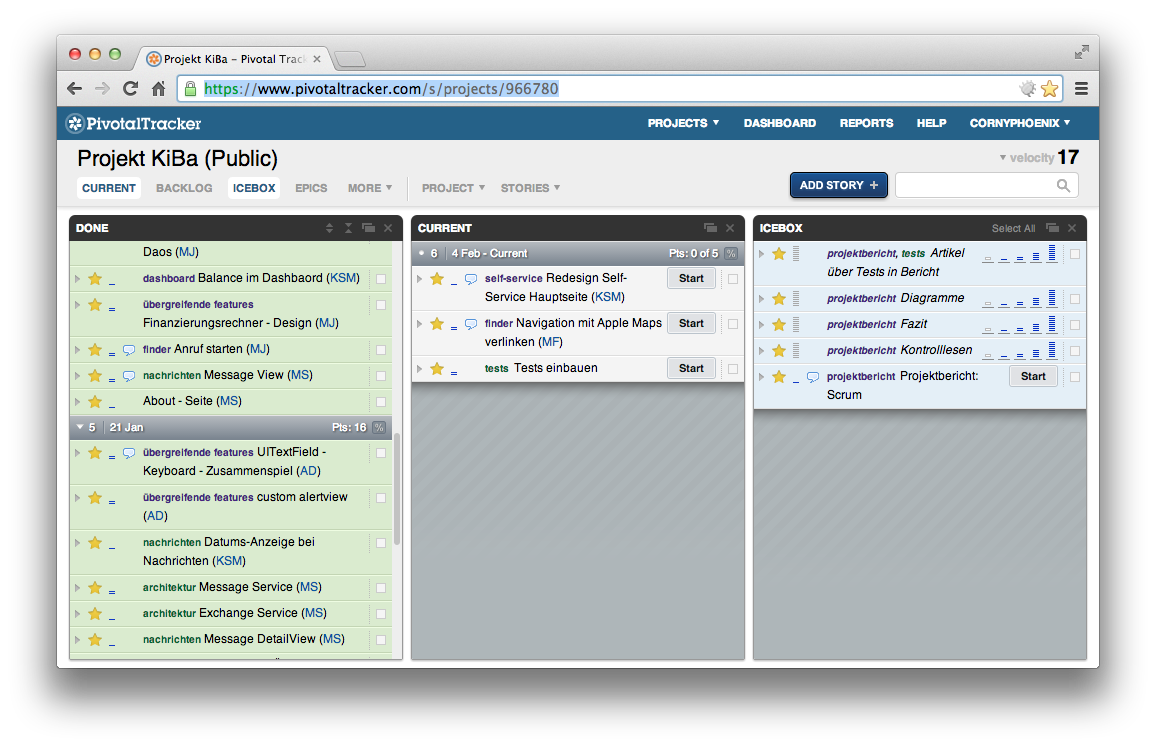
\includegraphics[scale=.3]{Pictures/TrackerStories}
	\vspace{-.8cm}
	\caption{Stories in PivotalTracker\label{fig:TrackerStories}}
\end{figure}
zum anderen allerdings auch Burndown-Charts, welche für das Vorgehen während der Scrum-Iterationen unabdinglich sind. Denn so können wir den Fortschritt unserer App messen und haben ein Monitoring für die Entwicklung unserer Features, wie in Abbildung \ref{fig:TrackerBurndown} zu sehen ist.

\begin{figure}[h]
	\centering
	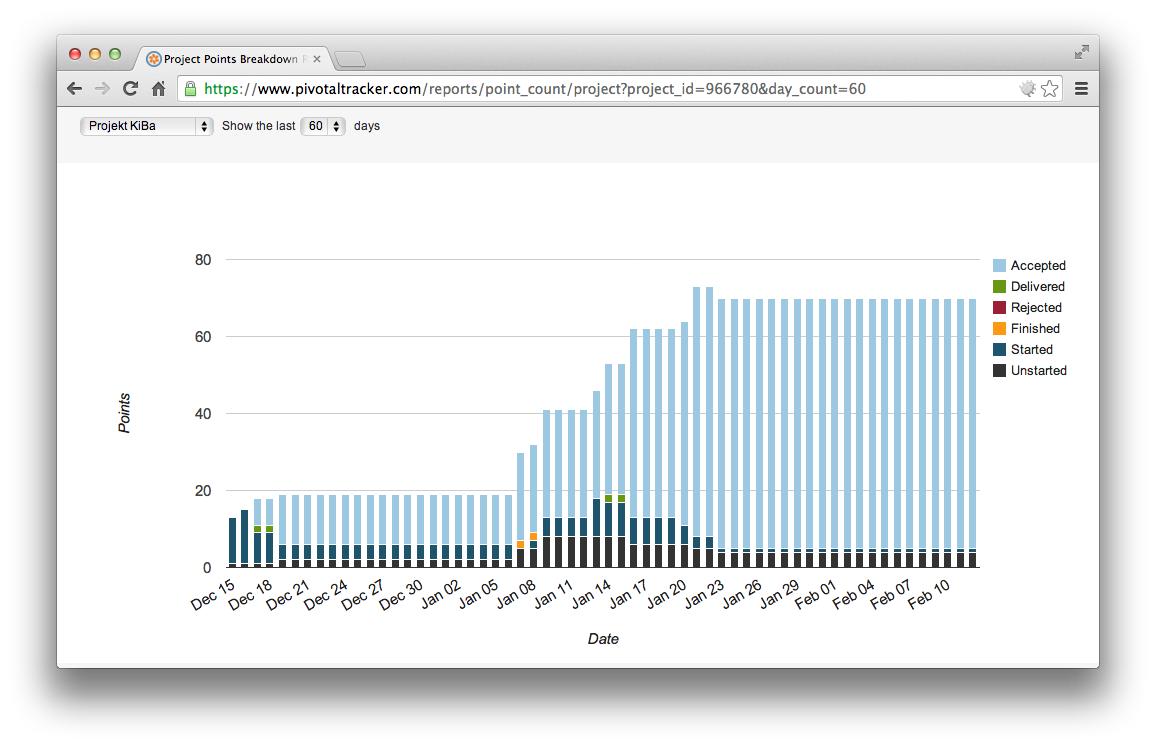
\includegraphics[scale=.3]{Pictures/TrackerBurndown}
	\vspace{-.8cm}
	\caption{Burndown-Chart in PivotalTracker\label{fig:TrackerBurndown}}
\end{figure}

\subsection{Quelltextversionierung}
GitHub + Git
\begin{figure}
	\centering
	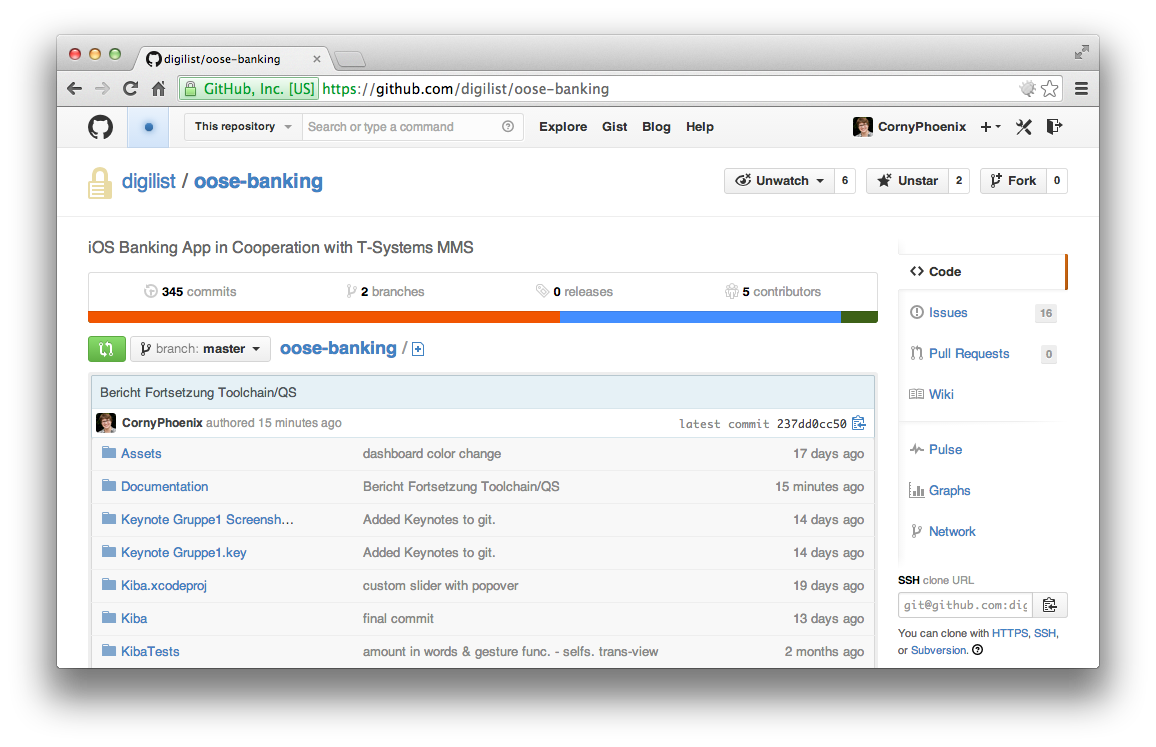
\includegraphics[scale=.3]{Pictures/GitHubOverview}
	\label{fig:GitHubOverview}
	\caption{Quelltext-Hosting bei GitHub}
\end{figure}
\begin{figure}
	\centering
	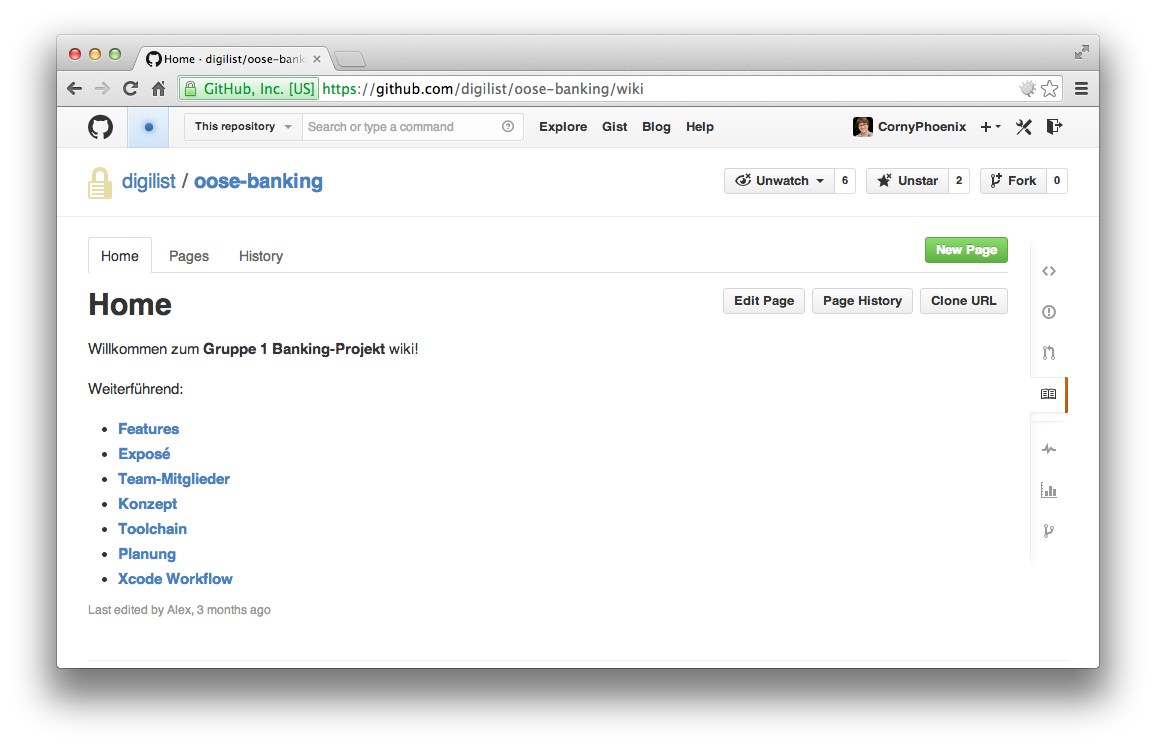
\includegraphics[scale=.3]{Pictures/GitHubWiki}
	\label{fig:GitHubWiki}
	\caption{GitHub-Wiki für den Wissensaustausch}
\end{figure}
\subsection{Konzept und erster Entwurf}
Balsamiq
\begin{figure}
	\centering
	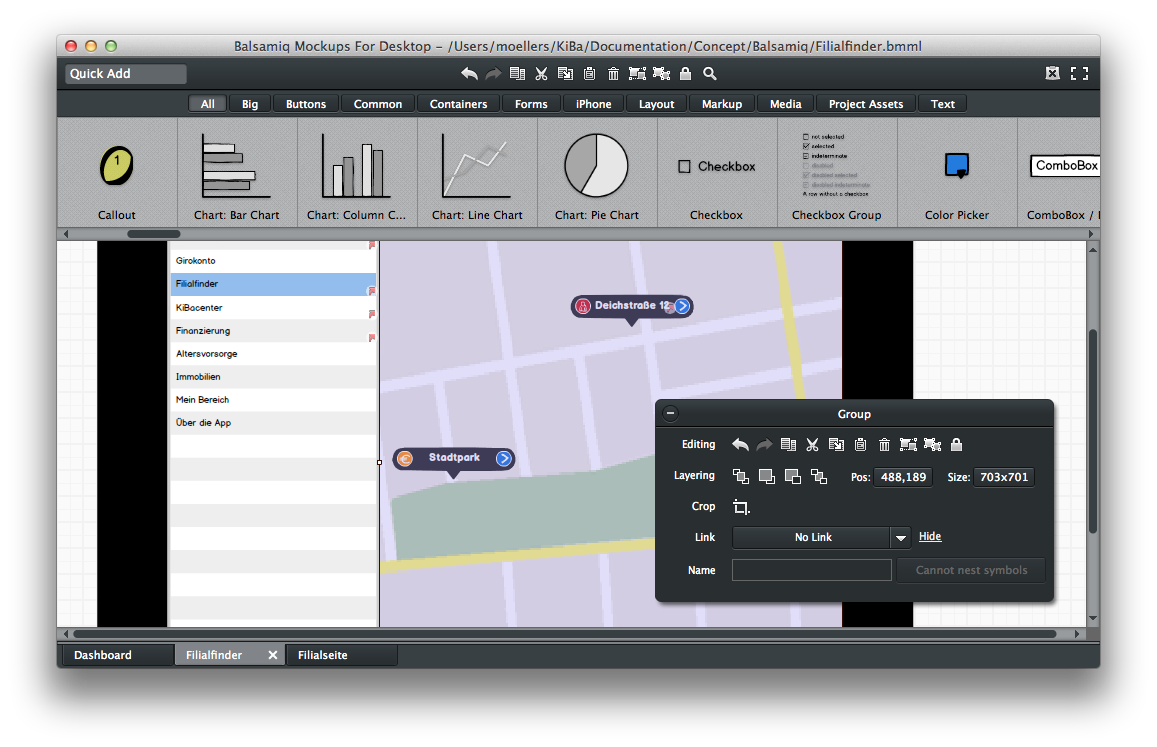
\includegraphics[scale=.3]{Pictures/BalsamiqEntwurf}
	\label{fig:BalsamiqEntwurf}
	\caption{Entwerfen mit Balsamiq}
\end{figure}
\subsection{Design- und Textsatztools}
Lua\LaTeX{}, Adobe Illustrator/Photoshop
\begin{figure}
	\centering
	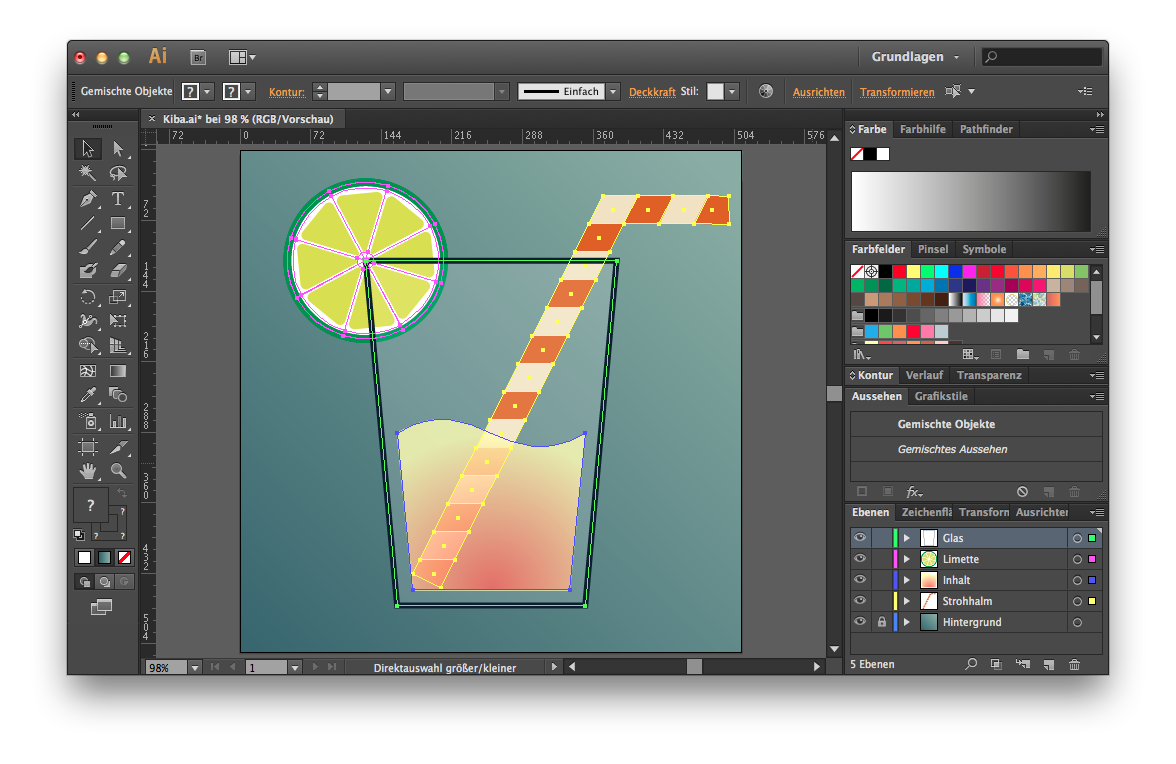
\includegraphics[scale=.3]{Pictures/IllustratorIcon}
	\label{fig:IllustratorIcon}
	\caption{Designen des KiBa-Icons mit Adobe Illustrator}
\end{figure}
\begin{figure}
	\centering
	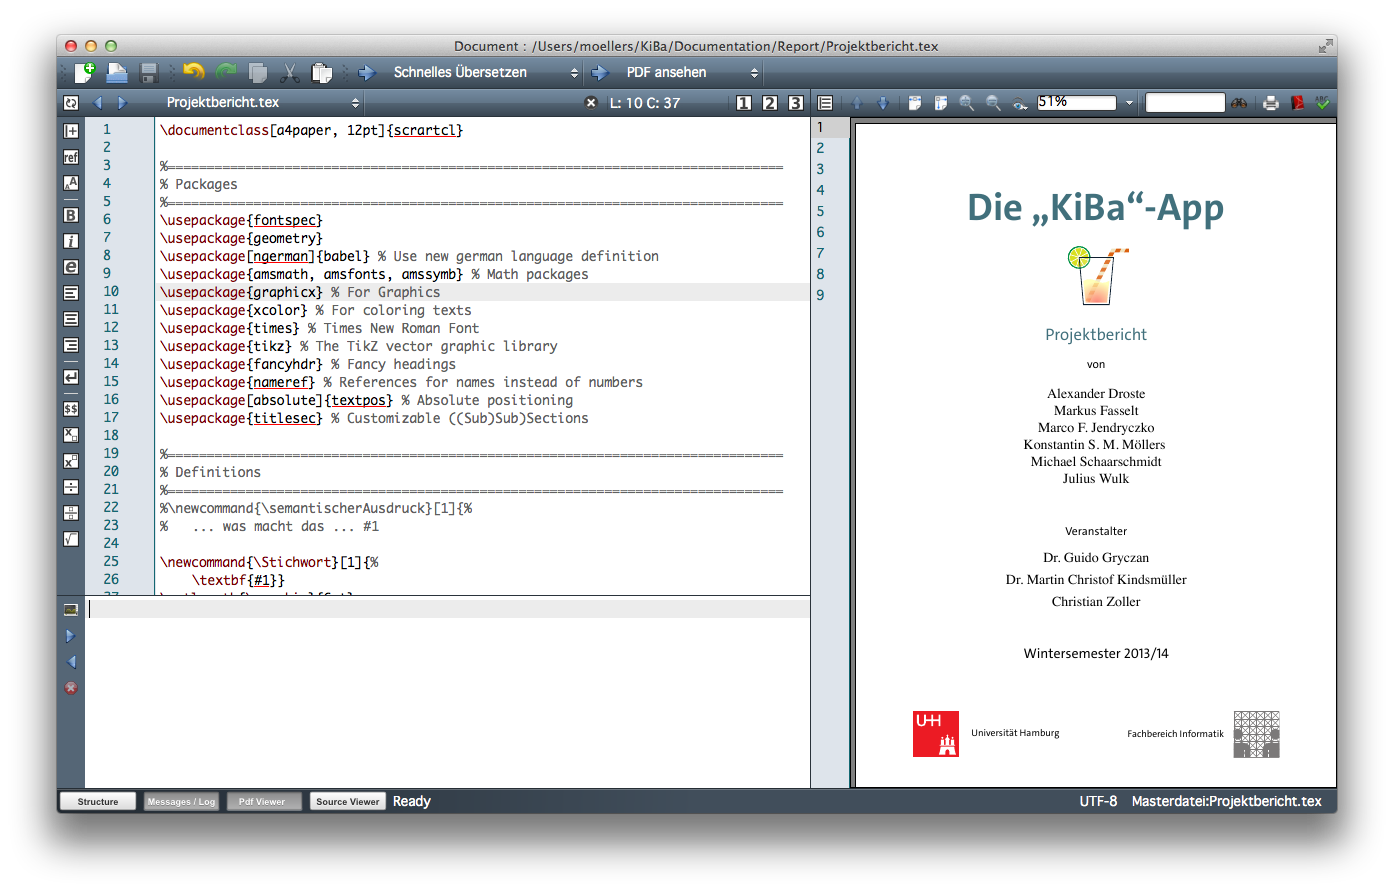
\includegraphics[scale=.3]{Pictures/LaTeXBericht}
	\label{fig:LaTeXBericht}
	\caption{Setzen des Projektberichts mit Lua\LaTeX}
\end{figure}